\documentclass[12pt,a4paper,oneside,brazil]{abntex2}
\usepackage[utf8]{inputenc}
\usepackage[T1]{fontenc}
\usepackage[brazil]{babel}
\usepackage{graphicx}
\usepackage{lipsum} % Pacote para gerar texto fictício
\usepackage{helvet}
\usepackage{ragged2e}
\usepackage{glossaries}
\usepackage[alf]{abntex2cite} % Citações padrão ABNT
\usepackage{indentfirst}
\usepackage{xpatch}
\usepackage{tabularx} % For flexible columns
\usepackage{blindtext}  % This package provides \blindtext
\usepackage{titlesec}   % This package is used for custom chapter title formatting
\usepackage{float}
\usepackage{fancyvrb}
\usepackage{listings}
\usepackage{caption}
\usepackage{acronym}

\setlength{\parindent}{1.5cm}

\renewcommand{\familydefault}{\sfdefault}

\hypersetup{
    hidelinks
}

\titulo{Plataforma de Edição/Automação para trabalhos acadêmicos}
\autor{Higor Ferreira Alves Santos}
\orientador{Marcelo Antônio Adad}

\newcommand{\ies}{Pontifícia Universidade Católica de Goiás}
\newcommand{\escola}{Escola Politécnica e de Artes}
\newcommand{\curso}{Engenharia de Computação}

\newcommand{\grauOrientador}{Prof. M.E.E.}
\newcommand{\grauAluno}{Bacharel}

\newcommand{\grauBancaUm}{Prof. Dra.}
\newcommand{\bancaUm}{Miriam Gusmão}
\newcommand{\grauBancaDois}{}
\newcommand{\bancaDois}{}

\instituicao{%
    \ies
    \par
    \escola
    \par
    \curso
}
\local{GOIÂNIA - GO}
\data{2024}

\newglossary*{abreviacao}{Lista de abreviaturas}
\newglossary*{sigla}{Lista de siglas}
\newglossary*{simbolo}{Lista de símbolos}

\newacronym[type=sigla]{api}{API}{Application Programming Interface}
\newacronym[type=sigla]{abnt}{ABNT}{Associação Brasileira de Normas Técnicas}
\newacronym[type=sigla]{css}{CSS}{Cascading Style Sheet}
\newacronym[type=sigla]{cms}{CMS}{Content Management System}
\newacronym[type=sigla]{dom}{DOM}{Document Object Model}
\newacronym[type=sigla]{ecma}{ECMA}{European Computer Manufacturers Association}
\newacronym[type=sigla]{xml}{XML}{eXtensible Markup Language}
\newacronym[type=sigla]{ies}{IES}{Instituição de Ensino Superior}
\newacronym[type=sigla]{mee}{M.E.E}{Mestre em Engenharia Elétrica}
\newacronym[type=sigla]{nbr}{NBR}{Norma Brasileira Regulamentadora}
\newacronym[type=sigla]{pucgo}{PUC-GO}{Pontifícia Universidade Católica de Goiás}
\newacronym[type=sigla]{pdf}{PDF}{Portable Document Format}
\newacronym[type=sigla]{svg}{SVG}{Scalable Vector Graphics}
\newacronym[type=sigla]{ssr}{SSR}{Server Side Rendering}
\newacronym[type=sigla]{spa}{SPA}{Single Page Application}
\newacronym[type=sigla]{tcc}{TCC}{Trabalho de Conclusão de Curso}
\newacronym[type=sigla]{ufpb}{UFPB}{Universidade Federal da Paraíba}
\newacronym[type=sigla]{ux}{UX}{User eXperience}
\newacronym[type=sigla]{ui}{UI}{User Interface}
\newacronym[type=abreviacao]{app}{App}{Application}
\newacronym[type=abreviacao]{bash}{bash}{Bourne Again Shell}
\newacronym[type=abreviacao]{cern}{CERN}{Conseil Européen pour la Recherche Nucléaire}
\newacronym[type=abreviacao]{xss}{XSS}{Cross-Site Scripting}
\newacronym[type=abreviacao]{xhtml}{XHTML}{eXtensible HyperText Markup Language}
\newacronym[type=abreviacao]{html}{HTML}{HyperText Markup Language}
\newacronym[type=abreviacao]{php}{PHP}{Hypertext Preprocessor}
\newacronym[type=abreviacao]{http}{HTTP}{Hypertext Transfer Protocol}
\newacronym[type=abreviacao]{js}{JS}{JavaScript}
\newacronym[type=abreviacao]{json}{JSON}{JavaScript Object Notation}
\newacronym[type=abreviacao]{jsx}{JSX}{JavaScript XML}
\newacronym[type=abreviacao]{latex}{LaTex}{Lamport TeX}
\newacronym[type=abreviacao]{mathml}{MathML}{Mathematical Markup Language}
\newacronym[type=abreviacao]{prof}{Prof}{Professor}
\newacronym[type=abreviacao]{regex}{RegEx}{Regular Expression}
\newacronym[type=abreviacao]{regexp}{RegExp}{Regular Expression}
\newacronym[type=abreviacao]{ts}{TS}{TypeScript}
\newacronym[type=abreviacao]{tsx}{TSX}{TypeScript XML}
\newacronym[type=abreviacao]{uuid}{uuid}{Universally Unique Identifier}
\newacronym[type=abreviacao]{UUID}{UUID}{Universally Unique Identifier}
\newacronym[type=abreviacao]{web}{Web}{World Wide Web}
\newacronym[type=abreviacao]{w3c}{W3C}{World Wide Web Consortium}


\makeglossaries
\DefineVerbatimEnvironment{createNextJsCommand}{Verbatim}
{numbers=left, numbersep=8pt, frame=single, framerule=0.5pt, firstnumber=1}
\DefineVerbatimEnvironment{promptNextJs}{Verbatim}
{numbers=left, numbersep=8pt, frame=single, framerule=0.5pt, firstnumber=1}
\DefineVerbatimEnvironment{yarnAddDpts}{Verbatim}
{numbers=left, numbersep=8pt, frame=single, framerule=0.5pt, firstnumber=1}
\DefineVerbatimEnvironment{layoutExample}{Verbatim}
{numbers=left, numbersep=8pt, frame=single, framerule=0.5pt, firstnumber=1}
\DefineVerbatimEnvironment{pageExample}{Verbatim}
{numbers=left, numbersep=8pt, frame=single, framerule=0.5pt, firstnumber=1}
\DefineVerbatimEnvironment{c05be23f77134574b1f7bb206e04f1b7}{Verbatim}
{numbers=left, numbersep=8pt, frame=single, framerule=0.5pt, firstnumber=1}
\DefineVerbatimEnvironment{Code00041357d26c4e96ba12ce0888e14159}{Verbatim}
{numbers=left, numbersep=8pt, frame=single, framerule=0.5pt, firstnumber=1}
\DefineVerbatimEnvironment{Code6d33a9496209429da690d0a4c003791e}{Verbatim}
{numbers=left, numbersep=8pt, frame=single, framerule=0.5pt, firstnumber=1}
\DefineVerbatimEnvironment{Code5818f59a8332420b971fbaf697f8997d}{Verbatim}
{numbers=left, numbersep=8pt, frame=single, framerule=0.5pt, firstnumber=82}
\DefineVerbatimEnvironment{Codea622d7da4d60496f97bfaab7c50d6d7b}{Verbatim}
{numbers=left, numbersep=8pt, frame=single, framerule=0.5pt, firstnumber=120}
\DefineVerbatimEnvironment{Code427e40d149c74ac7a8bd8f3347a09f70}{Verbatim}
{numbers=left, numbersep=8pt, frame=single, framerule=0.5pt, firstnumber=75}
\DefineVerbatimEnvironment{codeEscape}{Verbatim}
{numbers=left, numbersep=8pt, frame=single, framerule=0.5pt, firstnumber=1}
\DefineVerbatimEnvironment{processHTML}{Verbatim}
{numbers=left, numbersep=8pt, frame=single, framerule=0.5pt, firstnumber=1}
\DefineVerbatimEnvironment{processHTML2}{Verbatim}
{numbers=left, numbersep=8pt, frame=single, framerule=0.5pt, firstnumber=39}
\DefineVerbatimEnvironment{posProcess1}{Verbatim}
{numbers=left, numbersep=8pt, frame=single, framerule=0.5pt, firstnumber=1}
\DefineVerbatimEnvironment{ParagraphBlockCode}{Verbatim}
{numbers=left, numbersep=8pt, frame=single, framerule=0.5pt, firstnumber=37}
\DefineVerbatimEnvironment{HeaderBlockCode}{Verbatim}
{numbers=left, numbersep=8pt, frame=single, framerule=0.5pt, firstnumber=5}
\DefineVerbatimEnvironment{getParagraphCode}{Verbatim}
{numbers=left, numbersep=8pt, frame=single, framerule=0.5pt, firstnumber=1}
\DefineVerbatimEnvironment{getHeaderCode}{Verbatim}
{numbers=left, numbersep=8pt, frame=single, framerule=0.5pt, firstnumber=1}
\DefineVerbatimEnvironment{getImageCode1}{Verbatim}
{numbers=left, numbersep=8pt, frame=single, framerule=0.5pt, firstnumber=1}
\DefineVerbatimEnvironment{getImageCode2}{Verbatim}
{numbers=left, numbersep=8pt, frame=single, framerule=0.5pt, firstnumber=13}
\DefineVerbatimEnvironment{getListCode1}{Verbatim}
{numbers=left, numbersep=8pt, frame=single, framerule=0.5pt, firstnumber=1}
\DefineVerbatimEnvironment{getPageBreak1}{Verbatim}
{numbers=left, numbersep=8pt, frame=single, framerule=0.5pt, firstnumber=1}
\DefineVerbatimEnvironment{getTableBlock1}{Verbatim}
{numbers=left, numbersep=8pt, frame=single, framerule=0.5pt, firstnumber=1}

% Definindo um comando personalizado para o tamanho da fonte
\newcommand{\chaptersize}{\fontsize{12pt}{1.5}\selectfont}
% Definindo a formatação do capítulo
\titleformat{\chapter}{\normalfont\bfseries\chaptersize\MakeUppercase}{\thechapter}{1em}{}

\titleformat{\section}{\normalfont\bfseries\chaptersize}{\thesection}{1em}{}

\titleformat{\subsection}{\normalfont\itshape\bfseries\chaptersize}{\thesubsection}{1em}{}

\titleformat{\subsection}{\normalfont\itshape\bfseries\chaptersize}{\thesubsection}{1em}{}

\titleformat{\subsubsection}{\normalfont\chaptersize}{\thesubsubsection}{1em}{}

\titleformat{\subsubsubsection}{\normalfont\chaptersize}{\thesubsubsubsection}{1em}{}

% Alterando o título da lista de figuras
\renewcommand{\listfigurename}{Lista de Figuras}
% Alterando o título da lista de tabelas
\renewcommand{\listtablename}{Lista de Tabelas}
% Alterando o título do sumário
\renewcommand{\contentsname}{Sumário}

% Início do documento
\begin{document}

% Capa personalizada
\begin{capa}
    \center

    \OnehalfSpacing
    \ABNTEXchapterfont\bfseries{\textsc{\MakeUppercase{\imprimirinstituicao}}}

    \vfill

    % Incluir logotipo
    
\includegraphics[width=0.15\textwidth]{/home/higor/Documents/TCC/editor2/src/assets/logo.png}

    \vfill

    \ABNTEXchapterfont\bfseries{\MakeUppercase{\imprimirtitulo}}

    \vfill

    \MakeUppercase{\imprimirautor}

    \vfill

    \bfseries{\MakeUppercase{\imprimirlocal}}

    \bfseries{\MakeUppercase{\imprimirdata}}
\end{capa}

% Folha de rosto personalizada
\begin{folhaderosto}

    \centering

    \MakeUppercase{\imprimirautor}

    \vfill

    \ABNTEXchapterfont\bfseries{\MakeUppercase{\imprimirtitulo}}

    \vfill

    \justifying
    \noindent\hspace*{70mm}%
    \begin{minipage}{\dimexpr\textwidth-70mm}
        \textnormal{
            Trabalho de Conclusão de Curso apresentado à
            \escola, da \ies, como parte dos
            requisitos para a obtenção do título de \grauAluno\,em
            \curso.\\\\
            Orientador:\\
            \begin{flushright}
                \grauOrientador \imprimirorientador
            \end{flushright}
            Banca examinadora:\\
            \begin{flushright}
                \grauBancaUm \, \bancaUm
                \grauBancaDois \, \bancaDois
            \end{flushright}
        }
    \end{minipage}

    \vfill

    \centering

    \bfseries{\imprimirlocal}

    \bfseries{\imprimirdata}
\end{folhaderosto}

% Folha de aprovação
\clearpage
    \centering
    \MakeUppercase{\imprimirautor}

    \vfill

    \ABNTEXchapterfont\bfseries{\MakeUppercase{\imprimirtitulo}}

    \vfill

    \justifying

    \textnormal{Trabalho de Conclusão de Curso aprovado em sua forma final pela Escola Politécnica e de
    Artes, da Pontifícia Universidade Católica de Goiás, para obtenção do título de \grauAluno\,em
    Engenharia de Computação, em: \rule{8mm}{0.4pt}/ \rule{8mm}{0.4pt}/ \rule{16mm}{0.4pt}}

    \centering

    \vspace*{3cm}

    \begin{flushright}
    \rule{10cm}{0.4pt}\\
    \textnormal{Orientador: \grauOrientador \imprimirorientador}

    \vspace*{10mm}

    \rule{10cm}{0.4pt}\\
    \textnormal{Orientador1: \grauBancaUm \, \bancaUm}

    \vspace*{10mm}

    \rule{10cm}{0.4pt}\\
    \textnormal{Orientador2: \grauBancaDois \, \bancaDois}
    \end{flushright}

    \vspace*{6cm}

    \bfseries{\imprimirlocal}

    \bfseries{\imprimirdata}
\clearpage % Começa uma nova página para a folha de rosto

%Dedicatória
\centering
\ABNTEXchapterfont\bfseries{\textsc{\MakeUppercase{Dedicatória}}}\\
\vspace*{3cm}
\justifying
\normalfont
Dedico a Aquele que se assenta inerte no trono de glória, em algum lugar
remoto do Universo.

À Pátria amada,
vestida em sua pele de cordeiro. Que promove a bondade
e a justiça do alto de suas majestosas pirâmides sociais, sustentadas
sob os pilares de sal da ambivalência.


À minha família, autora das maiores alegrias e melancolias que a
vida pode trazer.

\vspace{10mm}

A Deus, à Pátria, à Família!

\vspace{20mm}

Ao meu pai: Euripedes Alves dos Santos; minha mãe: Maria
Aparecida Ferreira Gomes dos Santos; e minha irmã:
Sthefany Ferreira Alves dos Santos.

\vspace{10mm}

Em memória do meu avô: Gabriel Ferreira Gomes, falecido durante
o processo de escrita deste trabalho.

\vspace{10mm}

Em memória de minhas avós: Maria Tavares dos Santos e
Jesuína Pereira Gomes.

\vspace{10mm}

Às amizades de qualidade conquistadas, cujo julgo compartilhado
torna a caminhada mais leve.

\vspace{30mm}

(Melhorar isso aqui)
Às criaturas do Vale, cuja matéria de acolhimento e aceitação
as vezes é tão boa quanto as extremas opostas criaturas do Caminho.



\clearpage

%Agradecimentos
\centering
\ABNTEXchapterfont\bfseries{\textsc{\MakeUppercase{Agradecimetos}}}\\
\vspace*{3cm}
\justifying
\normalfont
% \lipsum[1]
\clearpage

%Epígrafe
\centering
\ABNTEXchapterfont\bfseries{\textsc{\MakeUppercase{Epígrafe}}}\\
\vspace*{3cm}
\justifying
\normalfont
% \lipsum[1-3]
\clearpage

%Resumo
\centering
\ABNTEXchapterfont\bfseries{\textsc{\MakeUppercase{Resumo}}}\\
\vspace*{3cm}
\justifying
\normalfont
% \lipsum[12-13]
\clearpage

%Abstract
\centering
\ABNTEXchapterfont\bfseries{\textsc{\MakeUppercase{Abstract}}}\\
\vspace*{3cm}
\justifying
\normalfont
% \lipsum[7]
\clearpage

\pagenumbering{roman}

\listoffigures   % Lista de Figuras
\clearpage

\listoftables    % Lista de Tabelas
\clearpage


\printglossary[type=siglas,title=LISTA DE SIGLAS]
\clearpage

\printglossary[type=abrev,title=LISTA DE ABREVIATURAS]
\clearpage

% Correção: Usar \tableofcontents para o Sumário
\tableofcontents
\clearpage



\pagenumbering{arabic}
\setcounter{page}{1}
\textual

\justifying
\normalfont


\chapter{Introdução}

Escrever um trabalho científico pode ser uma tarefa desafiadora. \cite{severino}
destaca a complexidade e o rigor necessários na elaboração de trabalhos científicos, que não
apenas envolvem o domínio do conteúdo específico, mas também a aderência às normas
técnicas para apresentação formal e formatação correta.

A Associação Brasileira de Normas Técnicas 
(\acrshort{abnt})
, é a entidade responsável por,
dentre outras, fornecer as normas que regulam o processo de criação de trabalhos acadêmicos.
A Norma Brasileira Regulamentadora 
(\acrshort{nbr})
 Nº 14724, por exemplo: Especifica os princípios
gerais para a elaboração de (teses, dissertações e outros), visando sua apresentação à
instituição (banca, comissão examinadora de professores, especialistas designados e/ou
outros)
\cite{abnt}.

Ademais, ainda com respeito aos trabalhos acadêmicos, não somente a
regulamentação da 
\acrshort{nbr}
14724 deve ser observada. Há ainda a 
\acrshort{nbr}
6023 que trata a respeito
da elaboração de referências e a 
\acrshort{nbr}
10520, que diz respeito às citações em documentos.

\cite{castro}, adverte que: "Em ciência, não pode haver uma
separação entre forma e conteúdo. Trata-se de uma separação fictícia, pois fica se conhecendo
o conteúdo pela forma."~ Ou seja: A forma do trabalho, sua apresentação, sua formatação e
todo o seu arranjo gráfico é tão importante quanto seu conteúdo. 
\cite{medeiros} vai
complementar essa visão, afirmando que a apresentação gráfica "\[...\] contribui para a
consecução de um trabalho capaz de atingir seu objetivo. Monografia realizada sem a
preocupação gráfica, em geral, acaba malsucedida."~

Em seu artigo, 
\cite{SilvaVitoria}
vão analisar as percepções e dificuldades dos
alunos de um curso superior em Tecnologia de Gestão em Recursos Humanos. Dentre suas
dificuldades, (dos alunos em questão), é destacada a questão da formatação do trabalho
acadêmico. Há também o fato de que as bancas avaliam os trabalhos baseadas em critérios da
própria Instituição de Ensino Superior (
\acrshort{ies}
), critérios estes que não estão necessariamente
presentes nas normas da \acrshort{abnt}, ou seja, há uma subjetividade presente que não é comum a
todas às \acrshort{ies} quanto a questão da formatação. Essa subjetividade contribui para a confusão dos
alunos, pois a \acrshort{ies} avaliará de acordo com aquilo que julga apropriado, o que muitas vezes
pode obscurecer o direcionamento do aluno ao redigir/formatar seu trabalho."~

\clearpage

\cite{santos}
em seu Trabalho de Conclusão de Curso
(\acrshort{tcc})
, também analisa as
dificuldades encontradas por egressos, desta vez do curso de Ciências Contábeis da
Universidade Federal da Paraíba
(\acrshort{ufpb}).
Em sua pesquisa é destacado que "Quanto a
formatação do trabalho com as normas da 
\acrshort{abnt}, \[...\], 60\% teve alguma dificuldade, inclusive
32\% teve muita dificuldade.", ou seja, a formatação do trabalho é um grande desafio presente
na vida de boa parte dos estudantes em processo de escrita.

\section{Objetivo}

Levando em consideração os problemas que os alunos de diversas instituições de ensino enfrentam ao elaborar seus respectivos
trabalhos (conforme apresentado acima), o objetivo deste instrumento é desenvolver uma plataforma web de alta
interatividade\footnote{Refere-se à capacidade de um sistema, aplicação ou interface de responder
        às ações do usuário de maneira eficaz e intuitiva}
e
inteligibilidade\footnote{Refere-se à clareza e compreensibilidade da interface, documentação e feedback fornecidos pelo
    sistema. Um software inteligível facilita o entendimento do usuário sobre como utilizá-lo e quais são os resultados de suas ações.},
de modo que o discente possa se preocupar apenas com o conteúdo. Os detalhes de formatação, de acordo com os padrões da
\acrshort{abnt}
e da
\acrshort{ies},
ficarão a cargo da própria plataforma.

A criação de um trabalho de
\acrshort{tcc}
se dará basicamente por três passos básicos: Escrita em blocos;
\textit{Parsing}\footnote{O termo Parsing, (do inglês: análise), será utilizado no
sentido de analisar e transformar algo em outra coisa.}
e
Documento em
\acrshort{pdf}
. A Figura\ref{fig:Passos para criar um documento} ilustra esse fluxo na linha do tempo.

\begin{figure}[H]
    \centering
    \caption{Passo a passo para criar um documento na plataforma}
    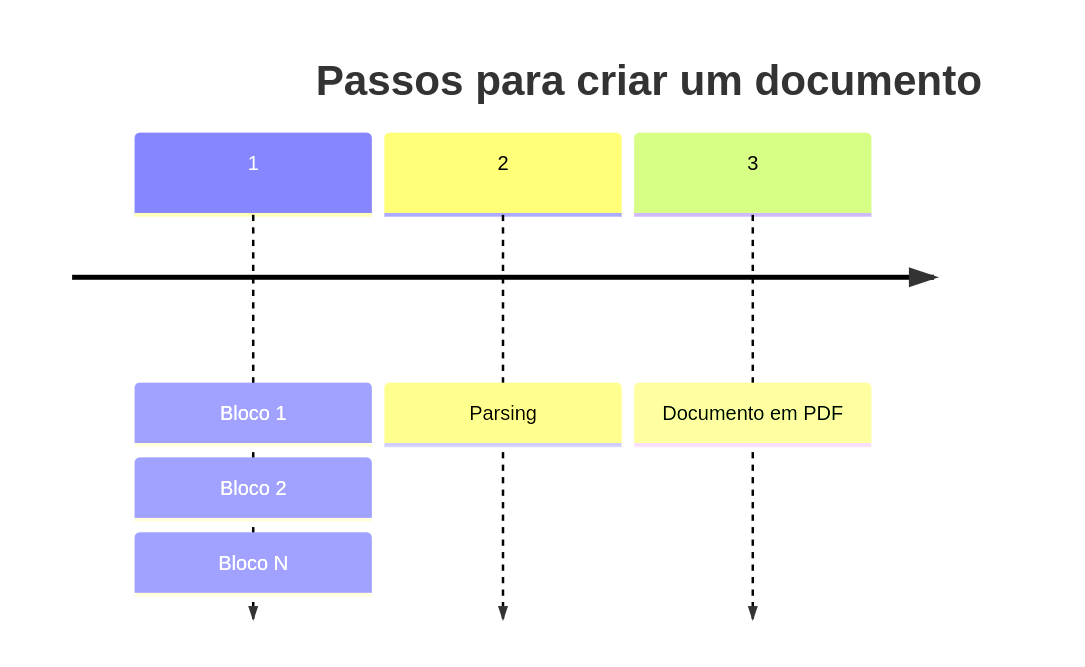
\includegraphics[width=0.8\textwidth]{./images/Passos para criar um documento.png}
    \label{fig:Passos para criar um documento} \\
    \textnormal{\fontsize{10pt}{12pt}Fonte: Autoria própria}
\end{figure}

O usuário interagirá com a aplicação escrevendo blocos que serão transformados
no documento final em
\acrshort{pdf}
. A este processo daremos o nome de Parsing. Após este, bastará
enviar o download do \acrshort{pdf}
ao usuário com todo o padrão de formatação. Os trabalhos desenvolvidos nesta plataforma
terão então duas versões: A versão de blocos, (sem formatação e interativa); e a versão
final já formatada em \acrshort{pdf}.

\section{Fluxo do documento}

\subsection{Escrita em blocos}

A escrita se dará de modo em que tudo será considerado um bloco.
A escrita em blocos consiste numa abordagem em que o texto vai sendo
escrito em seu fluxo natural, porém blocos podem ser adicionados à escrita.
Um bloco é um elemento adicionado ao fluxo de trabalho que desenpenha um papel
que o diferencia dos demais blocos.
Por exemplo: Uma imagem pode ser considerada um bloco nesta abordagem, uma vez
que não é um texto mas tem o objetivo de fornecer informações visuais. O próprio corpo
do texto em si será considerado um bloco, denominado parágrafo. Um título será um bloco
textual cujo objetivo será separar sessões do texto coesas. Uma lista será um bloco para enumerar
intens e assim por diante. O documento será basicamente uma composição de diversos blocos dispostos de forma a formar
uma unidade coesa final, que será o trabalho propiamente dito.

\subsection{Bloco}

Um bloco é uma unidade lógica no documento que desenpenha um papel especializado que nenhum
outro bloco o faz. Por exemplo: O bloco mais importante da
plataforma\footnote{O termo plataforma será utilizado
    de forma intercambiável e como sinônimo de aplicativo; sistema web; ou aplicativo da web}
será o de texto, (denominado bloco parágrafo), pois sem texto, não há trabalho.
Sem texto não há tão pouco comunicação que transmita informação
de caráter acadêmico-científico.

Semelhante ao bloco de texto, diversos outros blocos adjascentes
auxiliarão na construção do documento acadêmico. O bloco de imagem, por
exemplo, ajuda a exibir informações de forma ilustrativa e auxilia bastante
em exemplos que estão sendo dados em determinado contexto do texto.

A maior parte dos blocos contará com uma espécie de submenu, (em termos de aplicação),
que os permita personalizar. A personalização de blocos é importante para editar
configurações e dar autonomia ao usuário em determinar mais precisamente o papel
daquele bloco no texto. Por exemplo: Um bloco de título ajuda a separar o texto
em unidades coesas. Porém, existem diversos tipos de títulos: Existe o título, o
subtítulo, e até o subtítulo do subtítulo.

O submenu será a configuração que o usuário fará no bloco após escolhê-lo. No
caso do título, por exemplo: Após o usuário escolher este bloco, poderá configurar
o nível de título desejado. Nível este que varia do 1 ao 4, sendo 2; 3 e 4
espécies de subtítulos. No caso de uma imagem, o submenu funcionará para que possa
ser definida a imagem, bem como seu título de sua descrição.

A imagem abaixo ilustra a composição de um trabalho com seus respectivos blocos:

\begin{figure}[H]
    \centering
    \caption{Divisão de blocos em uma imagem}
    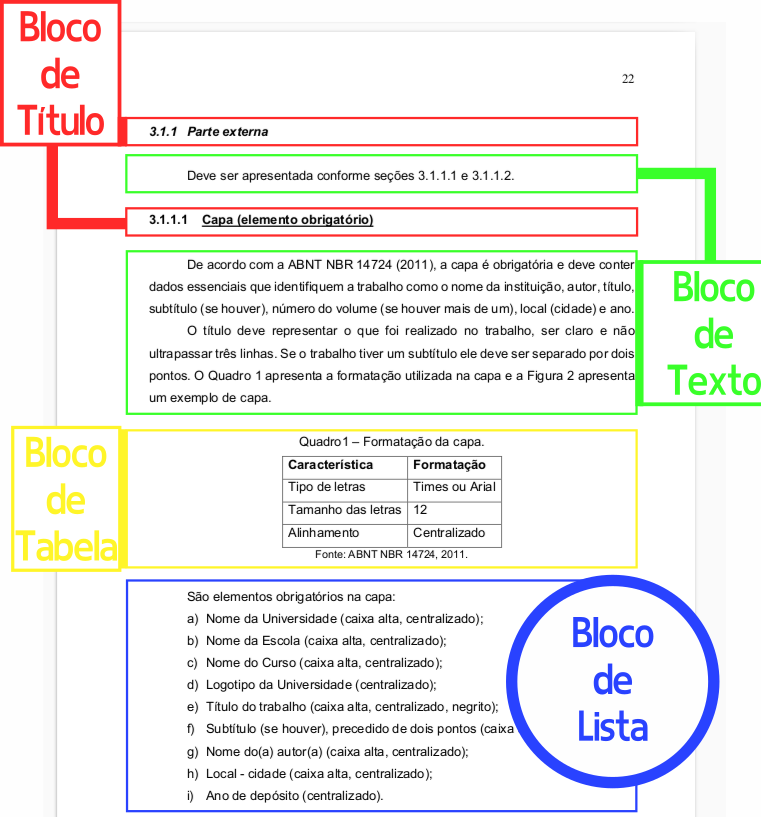
\includegraphics[width=0.8\textwidth]{./images/blocos-no-documento.png}
    \label{fig:blocos-no-documento} \\
    \textnormal{\fontsize{10pt}{12pt}Fonte: Adaptado de \cite{pucgo}}
\end{figure}

\subsection{Parsing}

O processo de Parsing é o processo que acontecerá sempre que o usuário desejar
ver o
\textit{layout}\footnote{Do inglês: Disposição, ou esboço. Esta palavra geralmente está associada ao desenho ou visual de algo.
}
da versão final de seu trabalho. Ele usa o código intermediário gerado pelos blocos para montar o
\acrshort{pdf}
final.

Este processo é, em termos simples, uma espécie de análise a ser aplicada no código gerado pelos blocos
da aplicação. A plataforma gerará um código
\acrshort{json}\footnote{Ver (sessão que trata do JSON)
}
como resultado das interações do usuário, que posteriormente
serão convertidos em código
\acrshort{latex}\footnote{Ver (sessão que trata do }.
Só então, finalmente será utilizado um utilitário que converterá o código \acrshort{latex}
em um documento
\acrshort{pdf}. A
Figura\ref{fig:app-json-latex-pdf} ilustra esse processo:

\begin{figure}[H]
    \centering
    \caption{Etapas do processo de Parsing}
    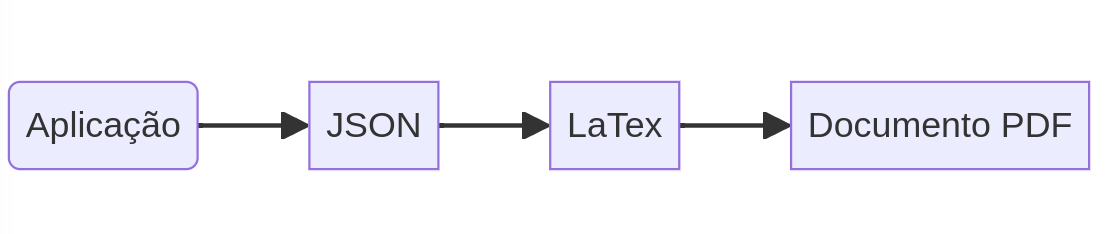
\includegraphics[width=0.9\textwidth]{./images/app-json-latex-pdf.png}
    \label{fig:app-json-latex-pdf} \\
    \textnormal{\fontsize{10pt}{12pt}Fonte: Autoria própria.}
\end{figure}

\section{Ambiente de desenvolvimento}

O ambiente de desenvolvimento é de extrema importância para que todas as ferramentas
utilizadas possam funcionar em perfeita harmonia em suas respectivas integrações e
colaborações. Muitas vezes, problemas de compatibilidade podem afetar
o funcionamento das mesmas e impedir que o programa final
seja executado corretamente, causando
\textit{bugs}\footnote{Do inglês: Inseto. Esta palavra é muito utilizada no contexto de desenvolvimento de aplicativos
para se referir a problemas que afetam o funcionamento dos mesmos
}
e outros imprevistos impeditivos tanto para a correta execução, quanto
para a exeperiência de desenvolvimento.
A lista abaixo diz respeito às ferramentas e ao ambiente onde este \textit{software}
foi desenvolvido, bem como todas as suas respectivas versões:

\clearpage

\subsection{Tecnologias do ambiente de desenvolvimento}

Atender aos requisitos mínimos de hardware
e software é fundamental para garantir uma experiência de usuário satisfatória
e evitar problemas de desempenho ou compatibilidade com o aplicativo da plataforma.
A seguir enumera-se o ambiente mínimo com seus respectivos softwares necessários
para rodar o aplicativo da plataforma:

\begin{table}[H]
    \centering
    \caption{Tecnologias do ambiente de desenvolvimento}
    \label{tbl:tecnologias-ambiente}
    \renewcommand{\arraystretch}{1.5}
    \begin{tabular}{p{6.4cm} p{9.6cm}}
        \hline
        \textbf{Tipo} & \textbf{Tecnologia} \\
        \hline
        Interpretador & NodeJs 20.10.0 \\
		Sistema Operacional & Ubuntu 20.04 \\
		Gerenciador de pacotes & Npm 10.2.3 \\
		Gerenciador de pacotes & Yarn 1.22.19 \\
		Utilitário & kpathsea version 6.3.4/dev \\
		Linguagem de Programação & TypeScript 5.3.3 \\
		Utilitário & BibTeX 0.99d (TeX Live 2022/dev/Debian) \\
		Navegador de Internet & Google Chrome 119.0.6045.199 \\
		Compilador & pdfTeX 3.141592653-2.6-1.40.22 (TeX Live 2022/dev/Debian) \\
		Utilitário & makeglossaries (Utilitário \acrshort{latex}) \\
        \hline
        \\\multicolumn{2}{c}{\fontsize{10pt}{12pt}Fonte: Autoria própria}
    \end{tabular}
\end{table}

\chapter{Fundamentação teórica}

A plataforma será construída sob alguns pilares fundamentais indispensáveis
a seu funcionamento. São estes pilares que garantirão o sucesso e o correto
funcionamento da aplicação, afim de que todo o objetivo discutido até o
presente momento seja atingido.

A
Figura\ref{fig:pilares-da-plataforma}
mostra em forma de mapa mental todos os principais pilares sobre os quais
o aplicativo será contruído. Estes pilares são formados por diversas
tecnologias, bibliotecas,
\textit{frameworks}\footnote{Uma framework é como um kit de ferramentas pré-pronto que fornece uma gama
    de funcionalidades pré-construídas e testadas afim de facilitar o processo
    de desenvolvimento. \cite{amazon-framework}
}
e conceitos que deverão trabalhar de forma integrada.

\begin{figure}[H]
    \centering
    \caption{Pilares da plataforma, (mapa mental)}
    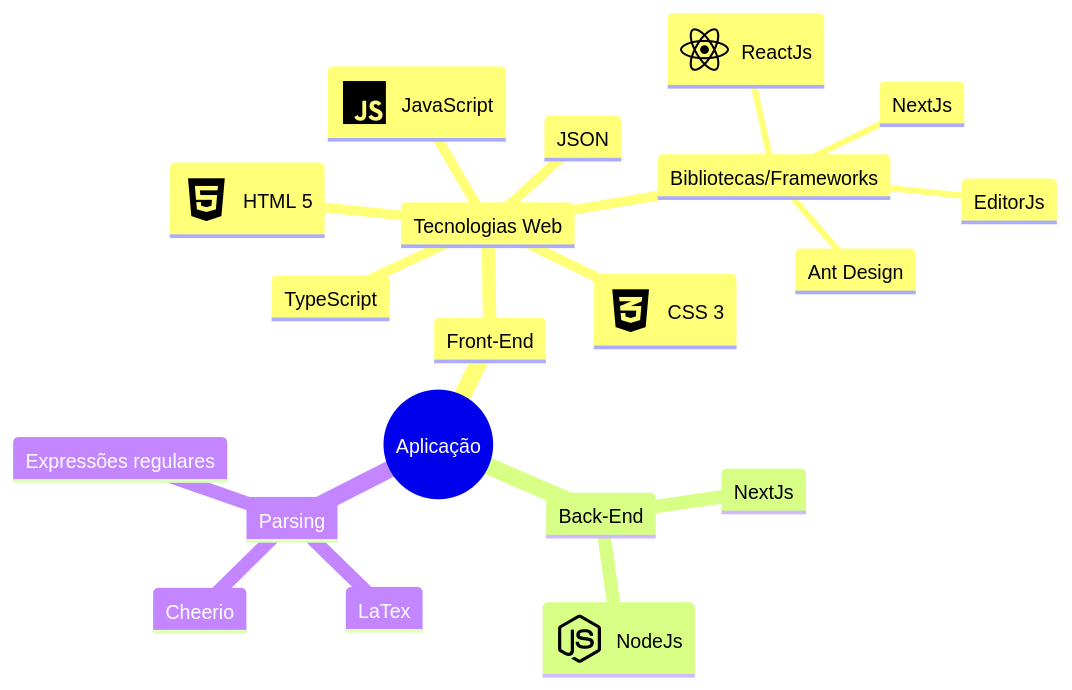
\includegraphics[width=0.9\textwidth]{./images/pilares-da-plataforma.png}
    \label{fig:pilares-da-plataforma} \\
    \textnormal{\fontsize{10pt}{12pt}Fonte: Autoria própria.}
\end{figure}

Estes pilares estão subdivididos em três grandes subcategorias, a saber: Front-End;
Back-End e Parsing. Cada qual com seus respectivos conceitos e tecnologias.

\section{Do Front-End}

O Front-End é, basicamente, a "linha de frente". É a parte da aplicação que interagirá
diretamente com o usuário. Ao profissional que codifica e desenvolve esta parte do
projeto, damos o nome de Desenvolvedor Front-End. A interface do usuário, que é
onde o mesmo realiza suas interações com o sistema, normalmente é desenhada por
um
\textit{designer}\footnote{Profissional que atua com design.
}
, ficando a cardo do desenvolvedor o papel de adaptar o
\textit{design}\footnote{Do inglês: Desenho.
}
ao código afim de obter os efeitos desejados.
\cite{totvs-front-end}

\subsection{Tecnologias Web}

As tecnologias
\acrshort{web}
desempenham um papel crucial na criação de experiências
digitais interativas, permitindo que os usuários se envolvam com o conteúdo de maneira mais
dinâmica e significativa. A incorporação da
\textit{Internet}\footnote{Rede mundial de computadores, \cite{marco-civil-art-2}.
}
na vida diária resultou em mudanças
significativas, marcada por um ritmo de evolução e aprimoramento sem precedentes, além da
distribuição de conteúdo em massa. Juntamente com essas mudanças, surgiram novas
tecnologias, variando de
\textit{softwares}\footnote{O software é o conjunto de instruções dadas a um computador, de modo que
    ele execute determinada tarefa. Podemos dizer que o software é
    a parte lógica do sistema computacional.  \\  \cite{hardware-e-software}.
}
a
\textit{hardwares}\footnote{Com hardware, compreende-se o equipamento físico de um sistema computacional.
    Suas unidades Lógicas de Processamento, memórias e unidades de armazenamento são
    hardware.  \\  \cite{hardware-e-software}.
},
aprimorando a experiência de navegação na
\acrshort{web}
\cite{molgado}.

A Internet, que teve origem nos Estados Unidos em 1969, foi inicialmente utilizada
por universidades, governos e instituições financeiras antes de se expandir globalmente. No
início, a internet era uma via de mão única onde os usuários consumiam informações e se
comunicavam de maneira privada. A evolução começou com a introdução de sistemas de
busca avançados, destacando-se o lançamento do Google em 1998, que democratizou o
acesso à informação.
\cite{vitoriano}.

A grande reviravolta na internet aconteceu em 1999, com o surgimento do
\textit{Blogger},
marcando o início da
Web
2.0, onde a comunicação tornou-se bidirecional. Os usuários
passaram a gerar conteúdo e se relacionar publicamente com marcas, empresas e pessoas por
meio de comentários, além de consumir informação. A evolução da tecnologia móvel, em
conjunto com o surgimento de redes sociais como
\textit{Fotolog},
\textit{MySpace},
\textit{Orkut},
\textit{Facebook},
\textit{YouTube}
e
\textit{Twitter},
ampliou o conceito de Web 2.0, permitindo o compartilhamento de fotos,
vídeos e textos em uma escala maior.
\cite{vitoriano}.

A forma como se interage com a internet também evoluiu ao longo do tempo.
Passou-se de sites estáticos para interativos e animados, chegando até aos sites totalmente
responsivos\footnote{A responsividade é a capacidade de uma página da
    \acrshort{web}
    em se adaptar a diferentes dispositivos e tamanhos de tela.
    \cite{responsivo}
}
e adaptáveis de hoje. Isso foi possível devido ao desenvolvimento de novos
gadgets e ao surgimento de novas linguagens de programação. Atualmente, a Web Moderna é
composta por várias técnicas, metodologias, linguagens e ferramentas que permitem o
desenvolvimento de aplicações conectadas e interativas, oferecendo diversas formas de
interação com interfaces digitais.
\cite{vitoriano}.

\subsubsection{\underline{Linguagem de Marcação de Hipertexto, HTML}}

A Linguagem de Marcação de Hipertexto, do inglês: HyperText Markup Language
(\acrshort{html})
foi criada por Tim Berners-Lee enquanto trabalhava na Organização Europeia para a
Pesquisa Nuclear
(\acrshort{cern}),
o laboratório de física de partículas na Suíça, no final dos anos
1980 e início dos anos 1990. O objetivo era criar uma maneira de compartilhar documentos e
informações em um ambiente de rede. A primeira versão do
\acrshort{html}
tinha apenas 18 elementos
de marcação, permitindo a formatação básica de texto e a inclusão de
\textit{links}\footnote{Do inglês: Ligação. Também chamado de hiperlink, é uma referência a um
    documento eletrônico que, quando clicado, leva o usuário para outro recurso
    ou documento.
},
imagens e listas.
\cite{w3c}.

O
\acrshort{html}
rapidamente ganhou popularidade e passou por várias iterações, cada uma
adicionando novos elementos e funcionalidades. O
\acrshort{html}4,
lançado em 1997, trouxe uma
série de melhorias, incluindo mais controle sobre a aparência das páginas web, a introdução
de folhas de estilo em cascata
(\acrshort{html})
e melhor suporte a
\textit{scripts}\footnote{Do inglês: Roteiro. Aqui usado no sentido de código fonte, que nada mais são
    do que um conjunto de instruções que o computador seguirá de modo interpretativo.
}.
\cite{w3c}.

Finalmente, o
\acrshort{html}5,
lançado oficialmente em 2014 pelo World Wide Web
Consortium (\acrshort{w3c}), trouxe uma série de novas funcionalidades, incluindo suporte nativo para
vídeo e áudio; novos elementos semânticos; gráficos e animações; geolocalização;
armazenamento local e muito mais.
\cite{w3c}.

\subsubsection{\underline{Funcionamento do HTML}}

O
\acrshort{html}
funciona como uma linguagem de marcação, o que significa que ele usa
\textit{"tags"}\footnote{Do inglês: Marcação.
}
para definir diferentes partes de um documento. Essas tags informam ao navegador
como exibir o conteúdo da página. Por exemplo, a tag
<p>
é usada para definir um parágrafo,
enquanto a tag
<h1>
é usada para definir um cabeçalho de primeiro nível.
\cite{w3c}.

As páginas
\acrshort{html}
são estruturadas usando uma combinação de elementos de bloco,
(que formam a estrutura principal da página), e elementos
\textit{inline}\footnote{Do inglês: Dentro da Linha. São elementos que podem ser escritos sem quebra de linha.
},
(que formatam o conteúdo
dentro desses blocos). Os elementos são aninhados dentro de outros elementos para criar a
estrutura hierárquica da página.
\cite{w3c}.

\subsubsection{\underline{HTML versão 5}}

Com o
\acrshort{html}5,
os desenvolvedores podem criar jogos online, reproduzir vídeos e
áudios diretamente no navegador, tudo isso sem a necessidade de instalação de plugins
externos. Isso resultou em uma melhor experiência geral do usuário, com carregamento mais
rápido e maior compatibilidade entre os navegadores.
\cite{w3c}.

Além disso, o
\acrshort{html}5
também trouxe recursos avançados de armazenamento local,
como o
\textit{\acrshort{web} Storage}\footnote{O termo
    \acrshort{web} Storage pode ser entendido, em tradução
    livre, como: Armazém da \acrshort{web}
}
e o
\textit{IndexedDB}\footnote{Termo abreviado de "Indexed DataBase", (Base de Dados Indexada).
}.
Esses recursos permitem que os sites armazenem dados
localmente no navegador do usuário, possibilitando a criação de aplicativos web
\textit{offline}
e
sincronização de dados em tempo real.
\cite{w3c}.

Outra contribuição importante do
\acrshort{html}5
é o suporte a tecnologias de
geolocalização e acesso aos recursos do dispositivo. Isso permite que os desenvolvedores
acessem informações de localização do usuário, câmera, microfone e acelerômetro, abrindo
possibilidades para o desenvolvimento de aplicativos web que utilizam esses recursos de
forma integrada.
\cite{w3c}.

Ao longo de sua história, o
\acrshort{html}
tem evoluído constantemente para acompanhar as
demandas e os avanços tecnológicos da web. O
\acrshort{html}5
é um marco significativo nessa
evolução, trazendo recursos semânticos, multimídia e interativos para a criação de páginas da
web modernas.
\cite{w3c}.

\subsubsection{\underline{Folhas de Estilo em Cascata, (CSS)}}

Folhas de Estilo em Cascata, ou \textit{Cascading Style Sheets}
(\acrshort{css}),
em tradução livre
para o português, é uma linguagem de estilo altamente eficaz e amplamente utilizada. Sua
principal função é definir a apresentação de documentos escritos em
\acrshort{html}
ou
\acrshort{xml}.
Isso
inclui uma série de linguagens baseadas em
\acrshort{xml},
como
\acrshort{svg},
\acrshort{mathml}
e
\acrshort{xhtml}.
O
\acrshort{css}
é
responsável por descrever a forma como os elementos são apresentados em diferentes mídias,
seja na tela do computador, em papel impresso, por meio de dispositivos de fala ou em outras
formas de mídia.
\cite{mdn-css}.

Considerado uma das principais linguagens da
Open\footnote{Do inglês: Aberto. Neste contexto, refere-se ao padrão "Aberto"~ da
    \acrshort{web}
}
\acrshort{web},
o
\acrshort{css}
tem uma grande
importância na padronização dos navegadores
\acrshort{web}.
Essa padronização é feita de acordo com
as especificações estabelecidas pela
\acrshort{w3c},
a organização que lidera a
\acrshort{web}
mundial. O
desenvolvimento do
\acrshort{css}
é feito em níveis distintos: o
\acrshort{css}1,
que hoje é considerado
obsoleto; o
\acrshort{css}2.1,
que atualmente é uma recomendação; e o
\acrshort{css}3,
que está sendo dividido
em pequenos módulos e caminha para a sua padronização.
\cite{mdn-css}.

\subsubsection{\underline{JavaScript}}

JavaScript é uma linguagem de programação notavelmente versátil que, apesar de ser
comumente conhecida pela sua utilização em páginas
\acrshort{web}, vai muito além disso.
Frequentemente abreviada para 
\acrshort{js}, essa linguagem é leve, interpretada e orientada a objetos
com funções de primeira classe. Graças à sua flexibilidade, o JavaScript se expandiu para uma
variedade de ambientes que não são navegadores, incluindo
Node.Js\footnote{Ver sessão que trata do Node.Js
},
Apache CouchDB\footnote{Base de dados que utiliza o JSON nativamente. Veja mais em:  \\ https://couchdb.apache.org/\#about
}
e
Adobe Acrobat\footnote{Software que lê e converte arquivos em formato
    \acrshort{pdf}. Veja mais em:  \\ https://www.adobe.com/br/acrobat.html
},
demonstrando sua adaptabilidade e eficácia em diversos contextos.
\cite{mdn-js}.

Com sua estrutura baseada em protótipos, o JavaSript é uma linguagem dinâmica que
suporta múltiplos paradigmas de programação. Isso significa que, além de ser orientada a
objetos, ela também suporta estilos de programação imperativos e declarativos, como a
programação funcional. Essa capacidade de suportar diferentes estilos de programação torna o
JavaScript uma ferramenta poderosa e flexível para os desenvolvedores.
\cite{mdn-js}.

O padrão para JavaScript é o
\acrshort{ecma}Script.
Desde 2012, todos os navegadores
modernos oferecem suporte completo ao
\acrshort{ecma}Script 5.1. Mesmo os navegadores mais
antigos fornecem suporte, pelo menos, ao
\acrshort{ecma}Script 3. A sexta versão do
\acrshort{ecma}Script,
oficialmente chamada de
\acrshort{ecma}Script 2015 e inicialmente conhecida como
\acrshort{ecma}Script 6
ou ES6, foi publicada pela \acrshort{ecma} International
em 17 de junho de 2015. Desde então, as
especificações do
\acrshort{ecma}Script são lançadas anualmente, demonstrando o desenvolvimento
contínuo e o avanço dessa linguagem padrão.
\cite{mdn-js}.

\subsubsection{\underline{TypeScript}}

O TypeScript, as vezes abreviado como
\acrshort{ts}, é uma linguagem fortemente
tipada construída em cima do JavaScript,
\cite{ts-page}.
Typescript traz uma sintaxe adicional para o JavaScript de modo
que o mesmo possa suportar checagem de tipos estática.
Sem o \acrshort{ts},
fica difícil saber com quais tipos de dados estar-se a trabalhar
durante o processo de desenvolvimento, pois o JavaScript é uma
linguagem fracamente tipada. Os parâmetros das funções e variáveis
não possuem nenhuma informação, forçando os desenvolvedores
a recorrerem a todo momento à documentação ou intuir sobre
as tipagens.
Typescript resolve esse problema, permitindo tipar o código
de modo que erros possam ser reportados quando a tipagem estiver
incorreta, por exemplo: ao tentar-se passar uma
string\footnote{Do inglês: Corda, barbante ou fio. No contexto de programação,
    é usado como termo para cadeira de caracteres. O caractere é, na
    maioria das linguagens de programação, um tipo de dado. E textos
    são formados por estas cadeias denominadas strings,
}
para uma função que espera um número, TypeScript lançará um erro.
O JavaScript, por outro lado, permitirá a execução deste código
podendo gerar erros de tempo de execução.
\cite{ts-w3}.

O TypeScript possui um compilador, que nada mais é do que um
transpilador. Este transpilador é responsável por transformar o
código
\acrshort{ts} em
\acrshort{js}.
Desta forma, o código JavaScript resultante da
transpilação pode ser rodado em praticamente qualquer
navegador ou ambiente que suporte o JavaScript.

\subsubsection{\underline{JavaScript Object Notation, JSON}}

\textit{JavaScript Object Notation}, (Notação de Objeto JavaScript),
popularmente chamado de \acrshort{json}. É uma sintaxe para a serialização de
objetos do javascript. Com objetos do javascript, compreende-se seus tipos
de dados e valores, como: objetos; matrizes; números; strings; booleanos;
\textit{null}\footnote{Do inglês: Nulo. Neste contexto é um valor especial do JavaScript para
    representar a nulidade de um objeto/variável.
}
e
\textit{undefined}\footnote{Do inglês: Indefinido. Neste contexto é um tipo de dado do JavaScript
    para variáveis indefinidas.
}.
Apesar de baseado na sintaxe do JavaScript, distingue-se desta
no sentido da forma de escrita. A serialização é o processo
de converter dados estruturados, (ou objetos), em um formato que pode
facilmente ser armazenado e transmitido pela rede. O \acrshort{json}
basicamente converte os objetos JavaScript em strings. Uma caracteristica deste,
é que \acrshort{json} é legível tanto por humanos, quanto por máquinas,
(na maioria dos casos).
\cite{mdn-json}.

A
Tabela\ref{tbl:json-descs}
mostra as principais
diferenças entre o JavaScript e o JSON.

\begin{table}[H]
    \centering
    \caption{Diferenças entre o JavaScript e o JSON}
    \label{tbl:json-descs}
    \renewcommand{\arraystretch}{1.5}
    \begin{tabular}{p{5.6cm} p{10.4cm}}
        \hline
        \textbf{Tipos e valores JavaScript} & \textbf{Diferença para o JSON} \\
        \hline
        Objetos e Arrays & Os nomes das propriedades devem ser strings com aspas duplas; as vírgulas à direita são proibidas. \\
		Números & Zeros à esquerda são proibidos; um ponto decimal deve ser seguido por pelo menos um dígito. \\
		Strings & Apenas um conjunto limitado de caracteres pode ser escapado; certos caracteres de controle são proibidos; o separador de linha Unicode (U+2028) e o separador de parágrafo (U+2029) são permitidos; strings devem ter aspas duplas.
             \\
        \hline
        \\\multicolumn{2}{c}{\fontsize{10pt}{12pt}Fonte: \cite{mdn-json}.}
    \end{tabular}
\end{table}

\subsection{Bibliotecas e Frameworks}

\subsubsection{\underline{ReactJs}}

\begin{figure}[H]
    \centering
    \caption{Logotipo do React}
    
\includegraphics[width=0.8\textwidth]{./images/react-logotipo.png}
    \label{fig:react-logotipo} \\
    \textnormal{\fontsize{10pt}{12pt}Fonte: React Dev, disponível em: https://react.dev/}
\end{figure}

"Biblioteca para interfaces de usuário \acrshort{web} e nativas".
O React é uma biblioteca de JavaScript criada pelo Facebook para solucionar
desafios de manutenção e escalabilidade em suas aplicações. No início de 2011, a equipe de
desenvolvedores do Facebook enfrentava dificuldades em lidar com o crescimento da
aplicação de anúncios, que estava se tornando cada vez mais complexa e difícil de ser
mantida. O aumento no número de membros da equipe e de funcionalidades estava afetando
negativamente os processos da empresa. Com tantas atualizações em cascata, a aplicação
estava se tornando lenta e difícil de ser atualizada sem falhas.
\cite{morais-react}.

Para resolver esses problemas, Jordan Walke, engenheiro do Facebook, propôs uma
solução inovadora. Ele sugeriu levar o 
XHP,
uma versão do
\acrshort{php},
para o navegador usando
JavaScript. O 
XHP
era uma tecnologia desenvolvida para minimizar ataques de Cross-Site
Scripting
(\acrshort{xss})
em aplicações
\acrshort{web}
dinâmicas. No entanto, ele não era capaz de lidar com o
grande número de requisições necessárias para esse tipo de aplicação. Com o apoio de sua
equipe de gerenciamento, Jordan Walke conduziu um experimento de seis meses para
explorar essa ideia. O resultado desse experimento foi o surgimento do ReactJS.
\cite{morais-react}.

O ReactJS revolucionou o desenvolvimento de interfaces de usuário ao introduzir o
conceito de componentes reutilizáveis e a abordagem de renderização virtual. Com a
utilização de componentes, os desenvolvedores podiam criar e reutilizar peças de interface
independentes e isoladas, o que simplificava o desenvolvimento e manutenção do código.
Além disso, a renderização virtual permitia atualizações de interface eficientes, otimizando o
desempenho da aplicação. O ReactJS foi lançado como um software de código aberto em
2013, permitindo que desenvolvedores de todo o mundo o utilizassem em seus projetos.
\cite{morais-react}.

Desde então, o React ganhou uma imensa popularidade e se tornou uma das
principais ferramentas para o desenvolvimento de interfaces de usuário em aplicações web.
Sua abordagem declarativa, que permite descrever como a interface deve ser exibida com
base no estado da aplicação, simplifica a construção de interfaces complexas. Além disso, a
capacidade de reutilização de componentes economiza tempo e esforço durante o
desenvolvimento. O React também influenciou o desenvolvimento do React Native, uma
versão da biblioteca voltada para a criação de aplicativos móveis multiplataforma. Com a
ajuda de uma grande comunidade de desenvolvedores e empresas, o ecossistema do React
continua a evoluir e fornecer soluções inovadoras para o desenvolvimento de interfaces de
usuário modernas e eficientes.
\cite{morais-react}.

O React teve seus primeiros sinais em 2010, quando o Facebook introduziu o XHP
na sua stack de
\acrshort{php},
permitindo a criação de componentes compostos. Em 2011, Jordan
Walke criou o FaxJS, protótipo inicial do React, que foi desenvolvido para resolver os
desafios de suporte aos anúncios do Facebook. Em 2012, o Instagram foi adquirido pelo
Facebook e expressou interesse em adotar o React. Isso levou o Facebook a dissociar o React
da empresa e torná-lo open source. Em 2013, ocorreu o lançamento oficial do React, mas
inicialmente enfrentou resistência da comunidade de desenvolvedores. No entanto, uma "turnê
do React"~ foi realizada para conquistar os não adeptos.
\cite{morais-react}.

No ano seguinte, o React começou a ganhar reputação e confiança. O
\textit{React Developer Tools}\footnote{Ferramentas de Desenvolvimento React
}
e o
\textit{React Hot Reloader}\footnote{Carregamento e recarregamento ultra rápido React
}
foram lançados, trazendo melhorias no
desenvolvimento e na experiência do usuário. Em 2015, o React se estabeleceu como uma
tecnologia estável, com empresas como Netflix e Airbnb adotando-o. O Redux, responsável
pelo gerenciamento de estado, foi lançado, e o React Native expandiu-se para o
desenvolvimento de aplicativos móveis para Android.
\cite{morais-react}.

Atualmente, o React continua evoluindo, com o lançamento de novas
funcionalidades e recursos para melhorar o desenvolvimento de aplicações. Iniciativas de
\acrshort{ssr}
\textit{(Server Side Rendering)}\footnote{Do inglês: Rederização do Lado do Servidor
}, e o foco em componentes funcionais são algumas das áreas de
desenvolvimento. O React permanece como uma biblioteca consolidada no mercado de Front-
End, sendo amplamente adotado por grandes empresas em todo o mundo.
\cite{morais-react}.

\subsubsubsection{JavaScript XML}

O JavaScript XML, (\acrshort{jsx}),
é uma extensão de sintaxe para o JavaScript que permite escrever
código de marcação, (como o \acrshort{html}),
dentro do JavaScript. Os componentes React nada mais são do que
funções ou classes chamadas a partir do código
\acrshort{js}
que atualizam o
\acrshort{html}
através da
\textit{Document Object Model}\footnote{Do inglês: Modelo de Documento de Objeto. O
    \acrshort{dom}
    é utilizado pelo JavaScript para manipular o documento
    \acrshort{html}
    exibido em tela.
    \cite{alura-dom}
 },
(\acrshort{dom}).
O
\acrshort{jsx}
facilita esse trabalho. Pois ao invés de chamar
funcões ou instanciar classes no código JavaScript,
pode-se escrever a marcação diretamente no mesmo,
como se o 
\acrshort{html}
estivesse dentro do
\acrshort{js}.
\cite{react-jsx}.

A
Figura\ref{fig:exemplo-jsx}
mostra um exemplo de código em
\acrshort{jsx}.
É exportada uma função denominada \textit{TodoList},
que nada mais é do que um componente React.
Esta função retorna um determinado valor, que é
o código
\acrshort{jsx}
propriamente dito. Este código será renderizado
no lugar onde esta função for chamada.

\begin{figure}[H]
    \centering
    \caption{Exemplo de código JSX}
    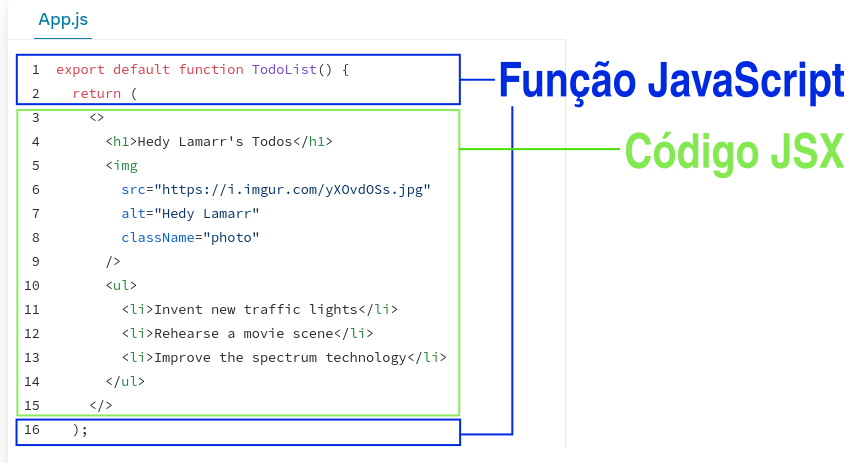
\includegraphics[width=0.9\textwidth]{./images/exemplo-jsx.png}
    \label{fig:exemplo-jsx} \\
    \textnormal{\fontsize{10pt}{12pt}Fonte: Adaptado de: ReactJs. Disponível em: <https://pt-br.react.dev/learn/writing-markup-with-jsx>}
\end{figure}

\subsubsection{\underline{NextJs}}

\begin{figure}[H]
    \centering
    \caption{Logotipo do NextJs}
    
\includegraphics[width=1.0\textwidth]{./images/nextjs-logotipo.png}
    \label{fig:nextjs-logotipo} \\
    \textnormal{\fontsize{10pt}{12pt}Fonte: Next.Js, disponível em: https://nextjs-template.vercel.app/}
\end{figure}

O NextJs é uma framework em ReactJs voltada à construção de aplicações
\acrshort{web}
tando na parte do Front-End quanto no Back-End.
Com NextJs, utiliza-se os componentes em React para construir as interfaces
de usuário, com o NextJs provendo recursos adicionais e otimizações.
\cite{nexjs-docs}.

NextJs também se encarrega de todas as configurações necessárias do React, como o processo
de
enpacotamento\footnote{Em inglês: Bundling. Um Bundle para a \acrshort{web},
    por exemplo, junta todos os códigos e recursos em um pacote otimizado
    para ser distribuído.
},
compilação e etc...
Permitindo ao desenvolvedor apenas focar no desenvolvimento da aplicação em si.
\cite{nexjs-docs}.

Devido à natureza desta framework, O NextJs é um pilar que aparece
tanto no Back-End quanto no Front-End. Estas duas frentes serão abordadas
com a utilização desta ferramenta, aproveitando ao máximo os recursos fornecidos
pela mesma. Os principais recursos oferecidos pelo NextJs são:

\begin{itemize}
        
	\item Roteamento: O NextJs provê um roteamento, (que é basicamente a navegação por páginas
                    dentro do app), baseado no sistema de arquivos do Sistema Operacional. Os arquivos
                    em pastas do projeto são mapeados para links, que fornecem os componentes de servidor
                    com suporte a
                    layouts\footnote{Layouts são como templates que são comuns às páginas roteadas. Ajudam no processo
                        de reaproveitamento de componentes pois eles podem ser extendidos às páginas,
                        que herdam características destes layouts.
                    },
                    rotas aninhadas, estados de carregamento, manipulação de erros,
                    entre outros...
                
	\item Renderização: NextJs fornece renderização do lado do cliente e do lado do servidor com
                    componentes de cliente, e componentes de servidor.
                
	\item Busca de dados: Há um processo de busca de dados simplificado com o uso de
                    \textit{async/await}\footnote{Recurso do JavaScript para lidar com a execuçao de código assíncrono.
                    }
                    nos componentes de servidor, além de uma
                    \acrshort{api}\footnote{Do inglês: Interface de Programação de Aplicações. É uma forma na qual
                        dois ou mais aplicativos ou componentes de de computador se comunicam
                        entre si. É uma interface de software que oferece um serviço para outras
                        partes do mesmo ou de outros softwares.
                        \cite{api-reddy}.
                    }
                    expandida para a memorização das
                    requisições,
                    \textit{caching}\footnote{O processo de caching é o ato de armazenar informações que são acessadas
                        frequentemente de maneira que seu acesso se torne mais rápido. Neste contexto,
                        o resultado de uma requisição pode ser armazenado em cache para que não
                        seja necessário consultar o servidor novamente quando a mesma informação
                        for requisitada.
                    }
                    de dados e revalidação.
                
	\item Estilização: Suporte para os métodos preferidos de estilização. Com inclusão
                    de: Módulos \acrshort{css}, \textit{Tailwind} \acrshort{css},
                    e \acrshort{css}-in-\acrshort{js}.
                
	\item Otimizações: Otimizações de scripts, imagens e fontes são também fornecidos para aprimorar
                    o núcleo do aplicativo e a experiência de usuário.
                
	\item TypeScript: Suporte total ao TypeScript, com uma melhor checagem de tipos e compilação eficiente.
                
    
\end{itemize}

\cite{nexjs-docs}.
            

\subsubsection{\underline{EditorJs}}

\begin{figure}[H]
    \centering
    \caption{Logotipo do EditorJs}
    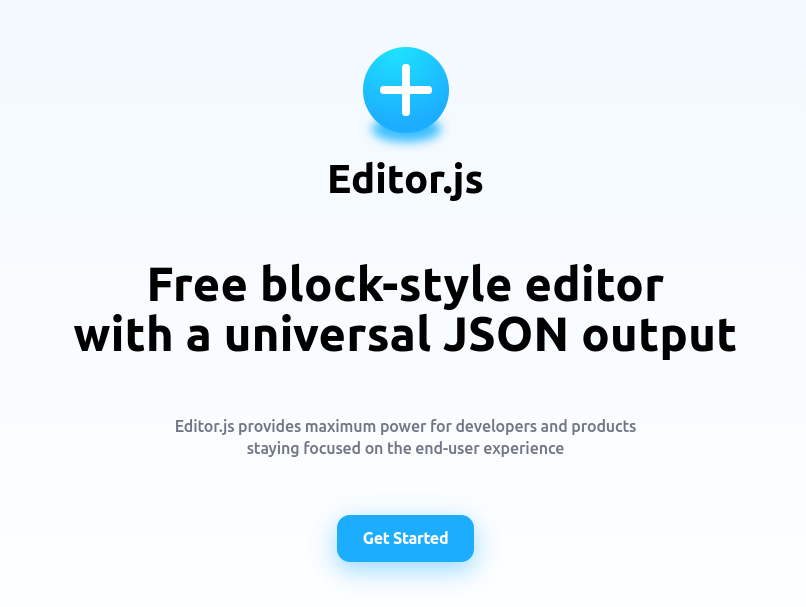
\includegraphics[width=0.8\textwidth]{./images/editorjs-logotipo.png}
    \label{fig:editorjs-logotipo} \\
    \textnormal{\fontsize{10pt}{12pt}Fonte: Editor.Js, disponível em: https://editorjs.io/}
\end{figure}

"Editor livre em blocos com saída universal em JSON".
O EditorJs é um rico editor de texto em blocos que oferece uma experiência de
edição intuitiva e versátil. Tudo o que é feito no EditorJs no fim é transformado
em um arquivo \acrshort{json} ao invés de um documento de marcação
em \acrshort{html}.
Essa abordagem deixa o processo mais simples para os desenvolvedores no
sentido de projetarem suas próprias integrações. Assim, o EditorJs pode ser
aplicado a diversas plataformas.
\cite{editorjs}.

São recursos do EditorJs:

\begin{itemize}
        
	\item Dados de saída limpos
	\item \acrshort{api} baseada em plugins
	\item Código aberto
    
\end{itemize}

O espaço de trabalho do EditorJs consiste em blocos separados, como:
Parágrafos; títulos; listas; etc... Cada um deles independentes entre si,
com muitos outros recursos como: Copiar e colar; seleção de vários blocos;
e entre outros que funcionam de forma familiar a outras ferramentas.
\cite{editorjs}.

O conceito chave do EditorJS é sua \acrshort{api}, na qual
todas as unides funcionais do editor são providas através de plugins externos que fazem
uso da mesma. Assim, o núcleo do EditorJs fica sendo mais abstrato e poderoso, de
modo que o desenvolvedor possa implementar diversos desafios com a criação
de seus próprios plugins.
\cite{editorjs}.

\subsubsection{\underline{AntDesign}}

\begin{figure}[H]
    \centering
    \caption{AntDesign}
    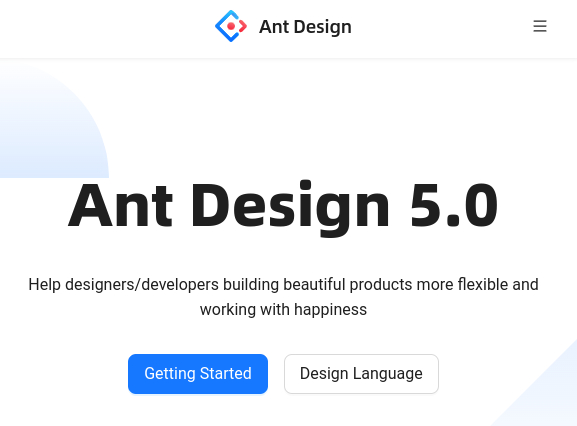
\includegraphics[width=0.8\textwidth]{./images/antdesign-pagina-inicial.png}
    \label{fig:antdesign-pagina-inicial} \\
    \textnormal{\fontsize{10pt}{12pt}Fonte: AntDesign, Disponível em: <https://ant.design>.}
\end{figure}

"Ajudando designers e desenvolvedores a construir belos produtos de forma flexível, trabalhando com alegria.".
O AntDesign é uma biblioteca de
\acrshort{ui},
\textit{User Interface}\footnote{Do inglês: Interface de Usuário
}.
Esta biblioteca é uma grande auxiliadora na hora de produzir aplicativos
com um design agradável sem que o desenvolvedor gaste muito tempo
estilizando os componentes da aplicação.

Totalmente integrado ao ReactJs, o AntDesign já traz consigo uma vasta
gama de componentes reutilizáveis que podem ser "encaixados"~ à
construção das telas do app.
O AntDesign não impacta somente a
\acrshort{ui},
mas também a
\textit{User Experience}\footnote{Do inglês: Experiância de Usuário
},
\acrshort{ux}, uma vez que seus componentes são construídos
em cima do React. Deixando-os altamente reativos e já com seus
devidos comportamentos padrão. Ficado a cargo do desenvolvedor
apenas personalizar o que se deseja fazer.
A
Figura\ref{fig:componente-ant-ex}
mostra um exemplo de implementação de um componente em AntDesign.

\begin{figure}[H]
    \centering
    \caption{Exemplo de componente em AntDesign}
    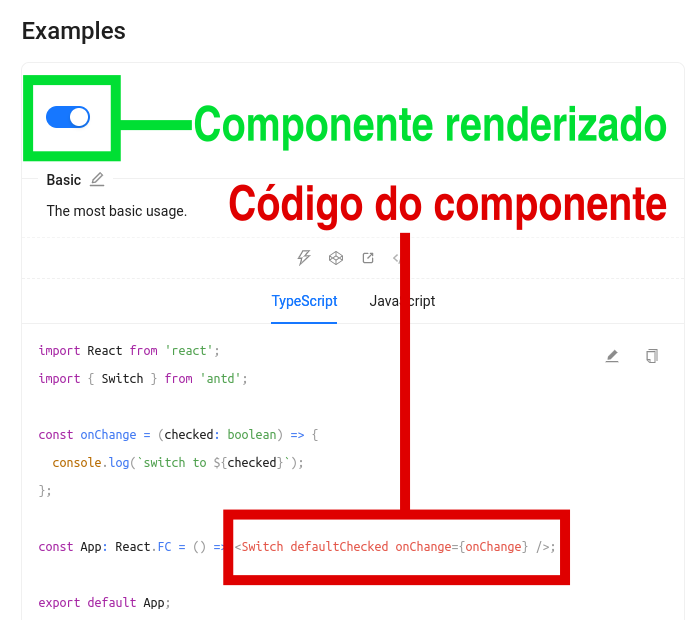
\includegraphics[width=0.9\textwidth]{./images/componente-ant-ex.png}
    \label{fig:componente-ant-ex} \\
    \textnormal{\fontsize{10pt}{12pt}Fonte: Adaptado de: AndDesign. Disponível em: <https://ant.design/components/switch>}
\end{figure}

Nota-se que com apenas uma linha tem-se um componente completo com
um visual totalmente moderno. Algo que com apenas
\acrshort{html},
\acrshort{css}
e
\acrshort{js},
gastaria algumas dezenas de linhas de código.
Tanto ReactJs quanto AntDesign significam economia
em termos de tempo, código e simplicidade de projeto.

\section{Do Back-End}

Back-end se relaciona com o que está por trás das aplicações desenvolvidas na programação. Ou seja, tudo que dá estrutura e apoio às ações do usuário da máquina é chamado de back-end. Quando acessamos um site, por exemplo, por trás de toda sua apresentação amigável esteticamente, há uma comunicação das informações trocadas entre banco de dados e navegador. Portanto, por trás da interface gráfica do realizador, o back-end está sempre agindo.
\cite{totvs-back-end}.

\subsection{NodeJs}

\begin{figure}[H]
    \centering
    \caption{Logotipo do NodeJs}
    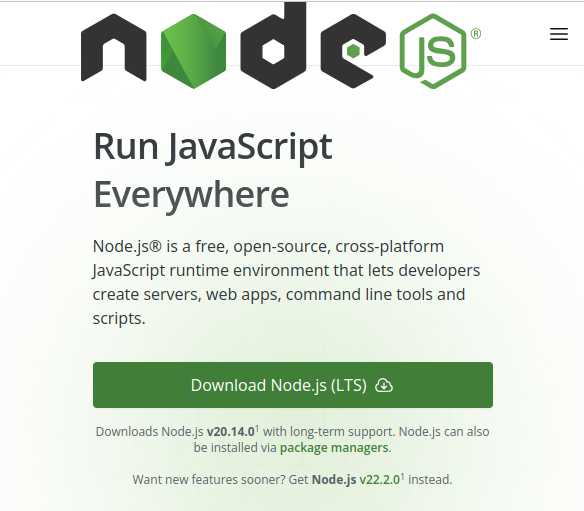
\includegraphics[width=0.7\textwidth]{./images/logotipo-nodejs.png}
    \label{fig:logotipo-nodejs} \\
    \textnormal{\fontsize{10pt}{12pt}Fonte: Adaptado de: NodeJs. Disponível em: <https://nodejs.org/en>}
\end{figure}

"Rode JavaScript em todo lugar".
O NodeJs é um ambiente de
\textit{runtime}\footnote{Do inglês: Tempo de execução. Um runtime é basicamente um interpretador
    capaz de executar um script.
}
que permite ao desenvolvedor criar servidores, aplicativos
\acrshort{web},
ferramentas e linha de comando, entre outros...
É a principal tecnologia deste projeto e o que permitirá
a execução de todas as outras na sequência.

Antes do NodeJs, o JavaScript era uma linguagem que
rodava puramente em
\textit{Browsers}\footnote{Do inglês: Navegadores. Aqui usado no sentido de
    navegador da \acrshort{web}, ou seja,
    o aplicativo no qual acessa-se páginas na internet.
}
como uma forma de adicionar interações às páginas da internet.
Com o NodeJs, o JavaScript passou do ambiente dos Browsers
ao ambiente dos Sistemas Operacionais. Abstraindo
\acrshort{api}s
dos mesmos. Hoje, com NojeJs, por exemplo, pode-se
acessar a
\acrshort{api}
do sistema de arquivos do Sistema Operacional.
Algo que há um tempo atrás só se fazia com
linguagens de baixo nível como o C++.

A plataforma desenvolvida neste trabalho será
um servidor que distribuirá o Sistema
\acrshort{web}
que é a plataforma em si. O NextJs,
tecnologia escolhida para este fim,
é um servidor capaz de processar uma parte
das interfaces do sistema estaticamente, e
entregá-las ao cliente juntamente com os scripts
de suas partes dinâmicas. Desta forma,
ganha-se segurança no processamento back-end
ao mesmo tempo que não perde-se em termos de
interatividade com o usuário.
Há também diversos ganhos de performance e simplificação
de código, uma vez que back-end e front-end
serão concentrados no mesmo lugar, não precisando
separá-los em projetos diferentes.

\section{O processo de Parsing}

O processo de Parsing é uma das partes mais vitais deste projeto.
Sem ele, não é possível obter o documento final formatado de acordo
com as normas postas da
\acrshort{abnt}
e da
\acrshort{pucgo}.
Pode-se dizer que o Parsing é o código núcleo da aplicação, pois todas
as outras partes, como edição em blocos e navegação, por exemplo,
serão feitas com o auxílio de bibliotecas e frameworks. O Parsing,
por sua vez, será escrito puramete em TypeScript para processar as
saídas do EditorJs.

Seu tratamento utilizar-se-á de uma combinação de expressões regulares
para tratar os caracteres especiais de código
\acrshort{latex},
manipulação de código
\acrshort{html}
produzido pelos plugins do editor utilizando-se o Cheerio.
E por fim, a compilação de código
\acrshort{latex}
utilizando-se o utilitário pdflatex
para gerar o
\acrshort{pdf}.

\subsection{Expressões regulares}

As expressões regulares, (as vezes denominadas
\acrshort{regex}
ou
\acrshort{regexp}),
podem ser descrevidas basicamente como uma sequência de
caracteres que descrevem um padrão de busca em um texto.
\cite{dp6-regex}.

Uma expressão regular pode ser composta por uma cadeia simples de caracteres, como
\textbf{abc};
ou uma cadeia composta pela combinação de caracteres simples e caracteres especiais.
Aos caracteres especiais, denominam-se metacaracteres. Os metacaracteres são usados
quando a busca no texto requer algo mais do que uma simples correspondência direta.
\cite{mdn-regex}.

\subsubsection{\underline{Expressão regular simples}}

No exemplo anterior, a expressão simples
\textbf{abc}
irá corresponder a uma letra
\textbf{"a"},
seguida de um
\textbf{"b"},
seguida de um
\textbf{"c"}
no texto ao qual se está avaliando.
Estas letras terão de estar juntas e nesta exata ordem.
Esta expressão irá encontrar correspondências nas strings
"Vamos aprender o abc do Regex?"~
e
"Um bug no sistema dói como um abcesso.".
Nestes dois casos, houve uma correspondência da substring
\textbf{abc},
mas a string
"ab c"~
não irá obter correspondência, pois aqui a exata substring
\textbf{abc}
não está contida. Observe as correspondências na
Figura\ref{fig:abc-match}.
\cite{mdn-regex}.

\begin{figure}[H]
    \centering
    \caption{Correspondêcias do Regex abc}
    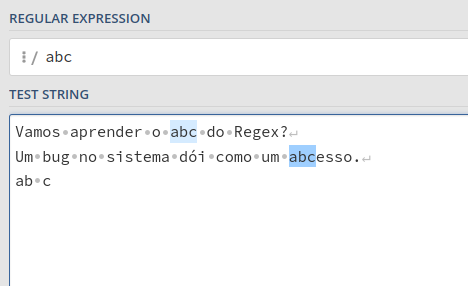
\includegraphics[width=0.8\textwidth]{./images/abc-match.png}
    \label{fig:abc-match} \\
    \textnormal{\fontsize{10pt}{12pt}Fonte: Autoria própria}
\end{figure}

\subsubsection{\underline{Expressão regular com metacaractere}}

Como mencionado anteriormente, quando se quer algo que é mais do
que uma simples correspondência direta, utilizam-se metacaracteres.
O caractere
\textbf{*}
é um metacaractere de expressão regular. Por exemplo:
\textbf{ab*c}
utiliza o
\textbf{*}
como metacaractere. A expressão
\textbf{ab*c}
deve ser lida como: Corresponda ao caractere
\textbf{a,}
seguido por zero ou mais caracteres
\textbf{b}s,
seguido por um caractere
\textbf{c.}
Usar
\textbf{*}
após o
\textbf{b}
significa: zero ou mais ocorrências do item anterior, no caso
\textbf{b.}
Como vemos na
Figura\ref{fig:abc-meta-match}
as strings "cbbabbbbcdebc", "abbbbc"~ e "ac"~
encontrarão correspondências. As strings "ab", "a"~ e "abbbbbb", por
outro lado, não encontrarão correspondências, conforme a
Figura\ref{fig:abc-meta-not-match}.
\cite{mdn-regex}.

\begin{figure}[H]
    \centering
    \caption{Correspondêcias do Regex ab*c, com metacaractere}
    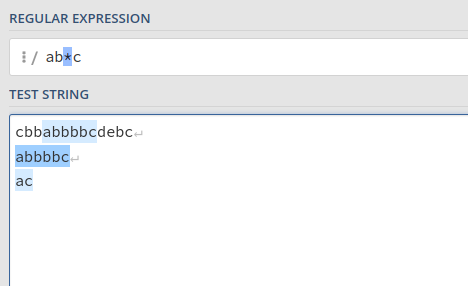
\includegraphics[width=0.8\textwidth]{./images/abc-meta-match.png}
    \label{fig:abc-meta-match} \\
    \textnormal{\fontsize{10pt}{12pt}Fonte: Autoria própria}
\end{figure}

\begin{figure}[H]
    \centering
    \caption{Não correspondêcias do Regex ab*c, com metacaractere}
    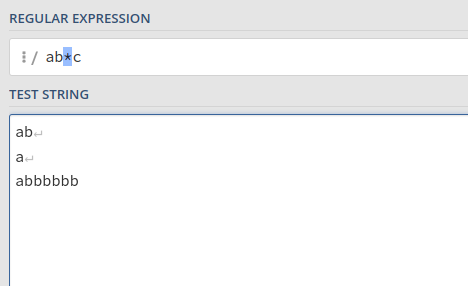
\includegraphics[width=0.8\textwidth]{./images/abc-meta-not-match.png}
    \label{fig:abc-meta-not-match} \\
    \textnormal{\fontsize{10pt}{12pt}Fonte: Autoria própria}
\end{figure}

Uma expressão regular é uma combinação de caracteres, alguns
deles, como o metacaractere quantificador *, visto
anteriormente, são caracteres especiais. Estes metacaracteres
são simbolos especiais que definem como a é interpretada.
\cite{dp6-regex}.

\subsubsection{\underline{Expressões regulares em JavaScript}}

Em JavaScript, as expressões regulares podem ser escritas diretamente dentro do código,
desde que postas entre barras //. Por exemplo: /abc/ é uma expressão regular válida em
\acrshort{js}.
O tipo de dados das expressões regulares é
o
\textit{object}\footnote{Do inglês: Objeto
}, assim como
\textit{Array}\footnote{Do inglês: Variedade ou matriz. No contexto de JavaScript é um dado estruturado,
    composto de uma sequencia de outros objetos ou dados puros.
}
ou
\textit{Set}\footnote{Do inglês: Conjunto. Assim como Array, é um dado estruturado que agrupa outros
    objetos, porém de forma não ordenada e não indexada.
}. As expressões regulares no
\acrshort{js}
são usadas com dois objetos principais, a saber
\acrshort{regex}
e
String.
A
\acrshort{api}
de strings do
\acrshort{js}
fornece uma gama de métodos nos quais podemos utilizar
juntamente com
\acrshort{regex}.
A Tabela\ref{tbl:string-methods-regex}
fornece uma descrição destes métodos:

\begin{table}[H]
    \centering
    \caption{Métodos de string que podem ser usados com regex}
    \label{tbl:string-methods-regex}
    \renewcommand{\arraystretch}{1.5}
    \begin{tabular}{p{2.4cm} p{13.6cm}}
        \hline
        \textbf{Método} & \textbf{Descrição} \\
        \hline
        match & O método match retorna o resultado da correspodência de um dado
            \cite{mdn-regex}
            à string ao qual está sendo aplicado. Aplicação em códido:
            "Meu abc".match(/abc/);
         \\
		matchAll & Faz o mesmo que match. Porém, ao contrário de match, que traz apenas
            a primeira correspondência, matchAll traz todas as correspondências
            encontradas.
         \\
		replace & O método replace de uma dada string, retorna uma nova string que substitui
            a correspondência de uma expressão regular por alguma string de substituição.
         \\
		replaceAll & Um caminho diferente para fazer o mesmo que replace, porém para todas
            as ocorrências.
         \\
		search & Faz uma busca pelo padrão na string e retorna o índice da primeira ocorrência. \\
		split & Divide a string em uma lista ordenada de substrings em que o critério de divisão é a expressão regular fornecida. \\
        \hline
        \\\multicolumn{2}{c}{\fontsize{10pt}{12pt}Fonte: \cite{mdn-regex}.}
    \end{tabular}
\end{table}

O objeto
\acrshort{regex}
também fornece dois métodos em que se usam as expressão regulares,
a saber: exec() e test().
\cite{mdn-regex}.

\subsection{Lamport Tex, LaTex}

\subsection{Cheerio}

\chapter{Desenvolvimento}

\begin{figure}[H]
    \centering
    \caption{Estrutura de pastas e arquivos básica do projeto}
    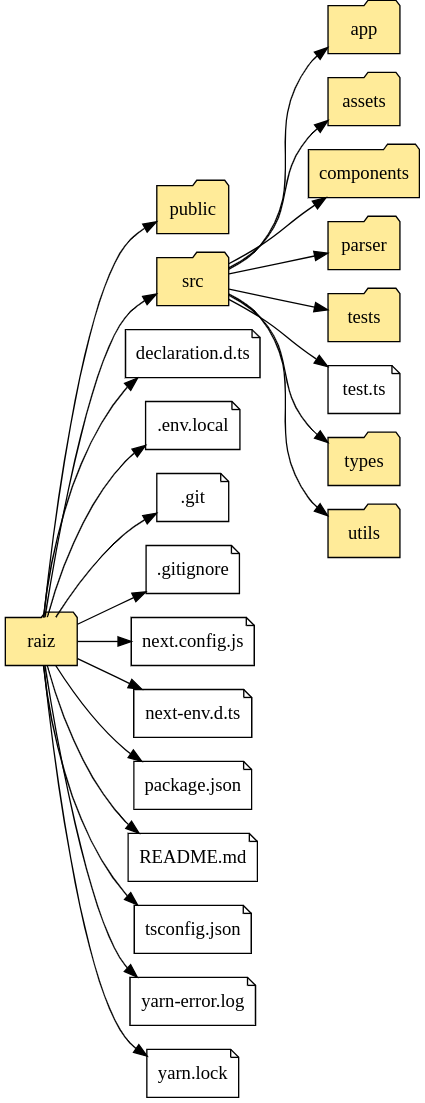
\includegraphics[width=0.4\textwidth]{./images/estrutura-basica-projeto.png}
    \label{fig:estrutura-basica-projeto} \\
    \textnormal{\fontsize{10pt}{12pt}Fonte: Autoria própria}
\end{figure}

\begin{table}[H]
    \centering
    \caption{Estrutura de pastas básica do projeto e suas atribuições}
    \label{tbl:pastas-projeto}
    \renewcommand{\arraystretch}{1.5}
    \begin{tabular}{p{3.2cm} p{12.8cm}}
        \hline
        \textbf{Arquivo/Pasta} & \textbf{Descrição} \\
        \hline
        public & Pasta pública para distribuição de arquivos estáticos. \\
		src & Esta pasta é onde praticamente todas as coisas na aplicação vão acontecer,
            aqui está as páginas e seus devidos roteamentos, o editor e seus plugins,
            o parser e tudo mais.
         \\
		declaration.d.ts & Arquivo de declarações. Aqui é anotado algumas tipagens para serem usadas
            globalmente durante o processo de desenvolvimento.
         \\
		.env.local & Arquivo de variáveis de ambiente para serem usadas como teste durante                o tempo de desenvolvimento \\
		.git & Pasta de controle do git. \\
		.gitignore & Arquivos a serem ignorados pela ferramenta de versionamento. \\
		next.config.js & Arquivo de configurações do NextJs \\
		next-env.d.ts &  \\
		package.json & Arquivo que define que o projeto é um projeto NodeJs. Aqui está toda a informação sobre dependencias
            do projeto, que são todos os pacotes usados de terceiros. Também possui definição
            de scripts úteis para serem utilizados no processo de desenvolvimento.
         \\
		README.md & Documentação de apresentação do projeto. \\
		tsconfig.json & Configurações do TypeScript. \\
		yarn-error.log & Erros do gerenciador de pacotes yarn \\
		yarn.lock & Arquivo de lock de dependências do gerenciador de pacotes yarn. \\
        \hline
        \\\multicolumn{2}{c}{\fontsize{10pt}{12pt}Fonte: Autoria própria}
    \end{tabular}
\end{table}

\section{NextJs e estrutura}

\section{EditorJS}

\subsection{Provider}

\subsection{Plugins}

\subsubsection{\underline{Classe base de plugin}}

\subsubsection{\underline{Plugin 1}}

\subsubsection{\underline{Plugin 2}}

\subsubsection{\underline{Plugin N}}

\section{Parsing, (parser)}

O processo de Parsing transformará cada bloco provido
pela saída do EditorJs em um trecho de código em
\acrshort{latex}.
Observe na
Figura\ref{fig:parsing-example-paragraph}
e
Figura\ref{fig:parsing-example-header}
os exemplos de parsing aplicados a um objeto de
\textit{Header}\footnote{Do inglês: Cabeçalho. Neste contexto, os headers são os títulos utilizados no documento.
}
e
\textit{Paragraph}\footnote{Do inglês: Parágrafo.
},
respectivamente.

\begin{figure}[H]
    \centering
    \caption{Parsing de um bloco Header}
    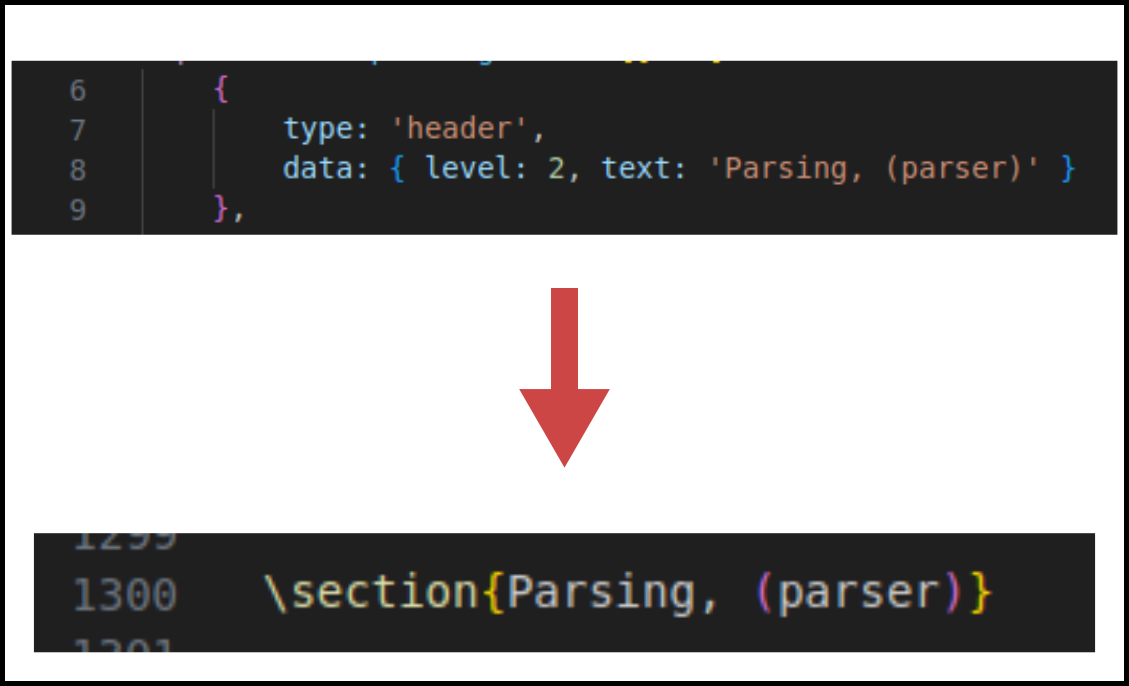
\includegraphics[width=0.8\textwidth]{./images/parsing-example-header.png}
    \label{fig:parsing-example-header} \\
    \textnormal{\fontsize{10pt}{12pt}Fonte: Autoria própria}
\end{figure}

\begin{figure}[H]
    \centering
    \caption{Parsing de um bloco Paragraph}
    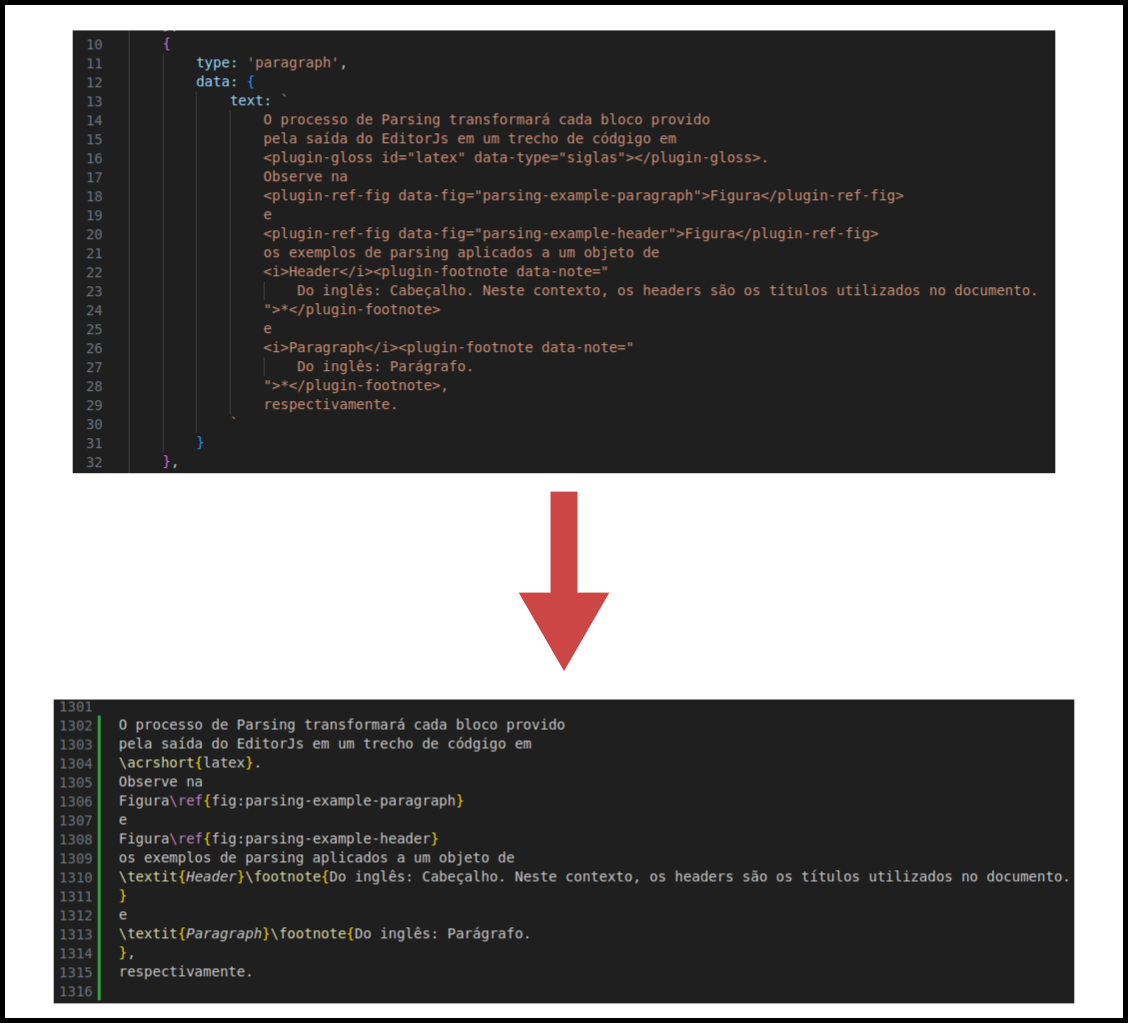
\includegraphics[width=0.8\textwidth]{./images/parsing-example-paragraph.png}
    \label{fig:parsing-example-paragraph} \\
    \textnormal{\fontsize{10pt}{12pt}Fonte: Autoria própria}
\end{figure}

No exemplo do bloco paragraph, é notável o processo de
processamento de
\acrshort{html}
acontecendo. Note que o conteúdo textual do bloco
não é apenas texto simples. Há quatro tags de
marcação personalizadas que se refletem em comandos
especiais
\acrshort{latex}, a saber:

\begin{enumerate}
        
	\item plugin-gloss
	\item plugin-ref-fig
	\item i
	\item plugin-footnote
    
\end{enumerate}

A tabela
Tabela\ref{tbl:plugins-latex-mapping}
mostra o mapeamento destas tags, que são plugins
\textit{in-line}\footnote{Do inglês: Em linha.
}
do EditorJs. As Tags possuem conteúdo e atributo, cada qual se
refletindo a uma particularidade do código
\acrshort{latex}
a depender de sua natureza.

\begin{table}[H]
    \centering
    \caption{Mapeamento de tags em código LaTex}
    \label{tbl:plugins-latex-mapping}
    \renewcommand{\arraystretch}{1.5}
    \begin{tabular}{p{1.92cm} p{1.92cm} p{1.92cm} p{3.2cm} p{7.04cm}}
        \hline
        \textbf{Tag} & \textbf{Conteúdo} & \textbf{Atributo} & \textbf{Valor do Atributo} & \textbf{LaTex} \\
        \hline
        plugin-gloss & Não & id & latex & \textbackslash acrshort\{latex\} \\
		plugin-ref-fig & Figura & data-fig & parsing-example-paragraph & \textbackslash ref\{fig:parsing-example-paragraph\} \\
		plugin-ref-fig & Figura & data-fig & parsing-example-header & \textbackslash ref\{fig:parsing-example-header\} \\
		i & Header & Não & Não & \textbackslash textit\{Header\} \\
		plugin-footnote & Não & data-note & <texto da nota> & \textbackslash footnote\{<texto da nota>\} \\
		i & Paragraph & Não & Não & \textbackslash textit\{Paragraph\} \\
		plugin-footnote & Não & data-note & Do inglês: Parágrafo. & \textbackslash footnote\{Do inglês: Parágrafo.\} \\
        \hline
        
    \end{tabular}
\end{table}

\subsection{Visão geral}

O parser da aplicação não depende de nenhuma biblioteca
ou framework de terceiros. O processo de parsing é feito
apenas utilizando-se de recursos nativos da linguagem
TypeScript, (consequentemente
\acrshort{js}).
A
Figura\ref{fig:estrutura-parser}
mostra a estrutura de pastas do módulo de parse, com três grandes
grupos:

\begin{itemize}
        
	\item process\_steps
	\item plugins
	\item mounting
    
\end{itemize}

O process\_steps diz respeito a funções utilitárias do processamento de texto.
É uma das mais importantes partes pois fornece funções que serão utilizadas a todo
momento em outras partes do parsing. Provê segurança pois nele reside as funções
de escape de caracteres especiais e entre outros.
O plugins fornece o processamento respectivo de cada plugin da aplicação,
e como cada um deverá ser convertido em código
\acrshort{latex}.
O mounting diz respeito a montagens de partes dinâmicas do documento
\acrshort{latex}.

\begin{figure}[H]
    \centering
    \caption{Estrutura de pastas do módulo de parse}
    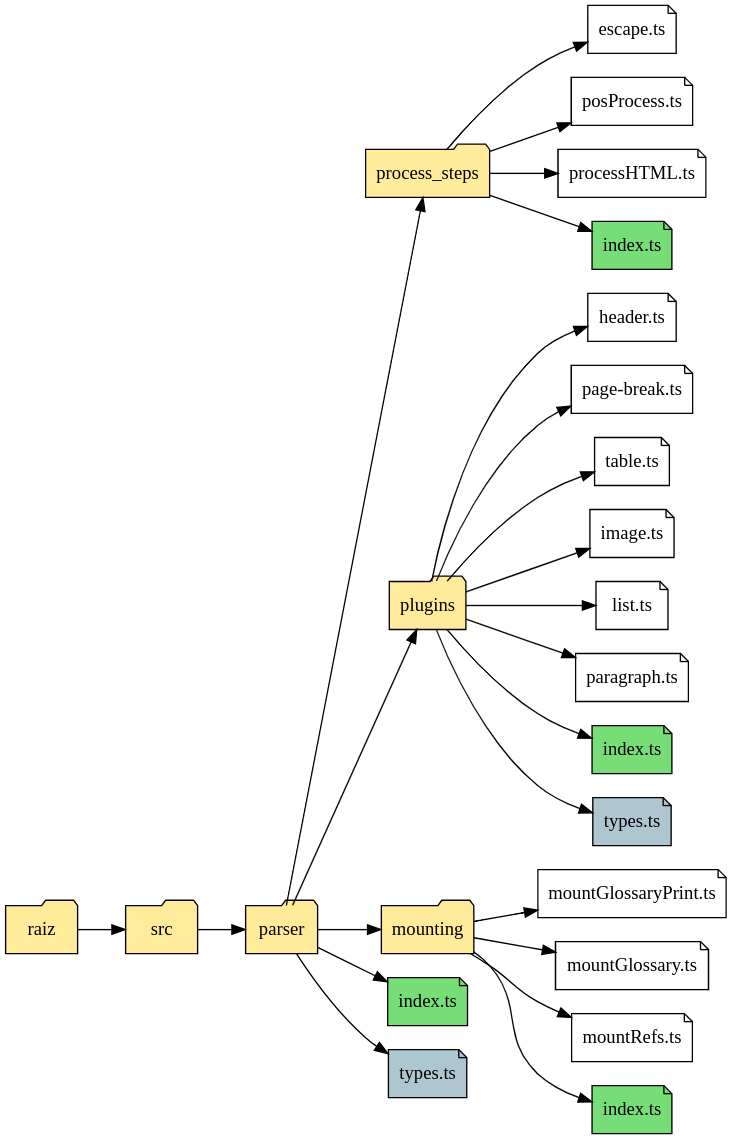
\includegraphics[width=0.8\textwidth]{./images/estrutura-parser.png}
    \label{fig:estrutura-parser} \\
    \textnormal{\fontsize{10pt}{12pt}Fonte: Autoria própria}
\end{figure}

\subsection{Estapas de processamento}

O principal plugin da aplicação a ser processado será o de paragraph.
A informação principal deste plugin é tão somente o texto de marcação
\acrshort{html}. Devido a este fato, este plugin
será o que mais utilizará as funções providadas pelo process\_steps.
A
Figura\ref{fig:fluxo-processamento-texto}
ilustra um ciclo de processamento de texto de marcação:

\begin{figure}[H]
    \centering
    \caption{Um ciclo de processamento de texto}
    
\includegraphics[width=0.9\textwidth]{./images/fluxo-processamento-texto.png}
    \label{fig:fluxo-processamento-texto} \\
    \textnormal{\fontsize{10pt}{12pt}Fonte: Autoria própria}
\end{figure}



\subsubsection{\underline{Escape de caracteres}}

O escape de processamento é a primeira etapa do processamento
de texto. Necessária para evitar o primeiro problema de transformar
o texto de marcação em código
\acrshort{latex},
que é o problema dos caracteres especiais.

O código
\acrshort{latex},
(como dito na fundamentação teórica),
é um código legível tanto para seres humanos
quanto por máquinas. Devido a isto, existem alguns caracteres
especiais de controle que ajudam a definir como
determinado conteúdo aparecerá no documento. Por exemplo:
O caractere \textbackslash~é  um dos mais importantes caracteres do latex, pois ele
define uma gama de comandos, como por exemplo o \textbackslash chapter\{\textbf{texto}\},
que define
\textbf{texto}
como sendo um capítulo no documento.
Mas e se o usuário digitar no documento um caractere \textbackslash ?

\subsubsection{\underline{Processamento de HTML}}

\subsubsection{\underline{Pós processamento}}

\subsection{Plugins}

\subsubsection{\underline{Tipagem}}

\subsubsection{\underline{Paragraph, (parágrafo)}}

\subsubsection{\underline{Header, (cabeçalhos)}}

\subsubsection{\underline{Image, (imagens)}}

\subsubsection{\underline{List, (listas)}}

\subsubsection{\underline{Page Break, (quebra de página)}}

\subsubsection{\underline{Table, (tabelas)}}

\subsection{Montagem}

\subsubsection{\underline{Glossário}}

\subsubsection{\underline{Referências}}


\bibliography{referencias}

\end{document}